\documentclass[letterpaper,12pt]{article}
\usepackage[spanish]{babel}
\spanishdecimal{.}
\selectlanguage{spanish}
\usepackage[spanish,onelanguage,ruled]{algorithm2e}
\usepackage[utf8]{inputenc}
\usepackage{graphicx}
\usepackage{caption}
\usepackage{subcaption}
\usepackage[top=2cm, bottom=2cm, left=2cm, right=2cm]{geometry}
\usepackage{hyperref}
\usepackage{verbatim}
\usepackage{amssymb}
\usepackage{mathtools}
\usepackage{listings}
\usepackage{color}
\definecolor{backcolour}{rgb}{0.95,0.95,0.92}
\newcommand\ddfrac[2]{\frac{\displaystyle #1}{\displaystyle #2}}
\lstset{backgroundcolor=\color{backcolour}, basicstyle=\footnotesize}
\lstset{xleftmargin=1cm, xrightmargin=1cm, breaklines=true}

\title{Práctica 6 \\ Lectura de un acelerómetro con la tarjeta Arduino y cálculo de velocidad}
\author{Laboratorio de Bio-Robótica}
\date{Construcción de Robots Móviles}
\begin{document}
\renewcommand{\tablename}{Tabla}
\maketitle
\section*{Objetivos}
\begin{itemize}
\item Utilizar el circuito MMA8452Q para medir la aceleración del robot móvil. 
\item Comunicar la tarjeta Arduino Uno con el acelerómetro mediante I2C.
\item Implementar un nodo de ROS en la tarjeta Arduino Uno que publique los valores del acelerómetro. 
\item Utilizar una interfaz gráfica de usuario (GUI) para desplegar los valores del acelerómetro. 
\item Implementar un filtro pasa-bandas para acondicionar la señal del acelerómetro.
\item Calcular una señal de velocidad mediante integración numérica. 
\end{itemize}

\section{Introducción}
Dependiendo del nivel de complejidad de la tarea que se pretenda resolver, un robot puede o no necesitar conocer su posición con respecto a algún sistema de referencia. Si la tarea no requiere de un alto nivel cognitivo, el comportamiento inteligente se puede lograr mediante la implementación de varios comportamientos y en general no es necesario conocer la posición del robot. Por el contrario, si la tarea implica la pleneación de rutas o el seguimiento de trayectorias, entonces sí es necesaria la posición del robot. 

El problema de determinar la posición del robot se conoce como localización y consiste en la obtención de la configuración del robot a partir de un mapa o alguna representación del ambiente y un conjunto de lecturas de los sensores. La odometría se refiere al cálculo de posición únicamente mediante la integración de velocidades o aceleraciones y se utiliza cuando no se dispone de un mapa o de los sensores adecuados. 

Cuando no se conoce la expresión analítica de una función se pueden utilizar métodos numéricos de integración. Uno de los más sencillos es el método del trapecio, en el cual la función es aproximada por una línea recta en un intervalo $[a,b]$ y la integral se aproxima con el área bajo la curva del trapecio que se forma. La señal que se desea integrar es la aceleración medida por el circuito MMA8452Q. Considere la aceleración en función del tiempo $a(t)$, cuya integral se desea obtener en el intervalo $[t_1,t_2]$. Por el método del trapecio se asume que
\[a(t) \approx  a(t_1) + \frac{a(t_2) - a(t_1)}{t_2 - t_1}(t - t_1)\]
por lo que la integral, es decir, la velocidad en el intervalo $[t_1,t_2]$, se puede obtener con
\[v(t) = \int_{t_1}^{t_2} a(t)dt \approx \frac{a(t_1) + a(t_2)}{2}(t_2 - t_1)\]
Puesto que los datos del acelerómetro se adquieren a una frecuencia constante, la diferencia $t_1 - t_2$ es constante y equivale al periodo de muestreo $\Delta t$. Reescribiendo la ecuación en términos discretos, la velocidad en el tiempo $k$ se puede obtener mediante:
\begin{equation}
v[k] = v[k-1] + \frac{a[k] + a[k-1]}{2}\Delta t
\label{eq:Integral}
\end{equation}

El circuito MMA8452Q es un acelerómetro de tres ejes y, a diferencia de una IMU (unidad de medición inercial), no cuenta con el hardware necesario para determinar su orientación. Las mediciones de aceleración siempre están alteradas por la fuerza de gravedad, es decir, las lecturas del acelerómetro son la suma de los efectos gravitatorios más la aceleración real del dispositivo. El vector de aceleraciones medidas en los tres ejes se puede modelar como
\begin{equation}
  \label{eq:accelModel}
  a_m = a_b - R_I^b \left[\begin{tabular}{c}0\\0\\g \end{tabular}\right]
\end{equation}
donde $a_m \in \mathbb{R}^3$ es el vector de aceleraciones medidas en los tres ejes XYZ, $a_b \in \mathbb{R}^3$ es el vector de aceleración real del sensor, $g$ es la aceleración de la gravedad y $R_I^b \in \mathbb{R}^{3\times 3}$ es la matriz de rotación que representa la orientación del sensor con respecto al sistema de referencia inercial. 

De la ecuación \ref{eq:accelModel} se puede observar que las mediciones del acelerómetro son altamente sensibles ante errores en la matriz de rotación $R_I^b$. Dado que el circuito MMA8452Q no cuenta con el hardware necesario para medir orientación, por lo que no se puede calcular con exactitud la matriz $R_I^b$, resultaría muy complicado obtener mediciones de posición a partir de la doble integración de la aceleración. Sin embargo, si se sabe que el robot sólo se moverá en el plano XY (perpendicular al vector de gravedad) y que los cambios en la aceleración en general serán lentos (por las características de los motores), se puede acondicionar la señal mediante filtros digitales para obtener una mejor estimación de la velocidad y posición. 

Un filtro digital es un sistema discreto cuyo propósito es reducir o mejorar ciertas componentes de una señal discreta. La reducción o amplificación generalmente se hace en términos de la frecuencia de la señal. En general, un filtro puede representarse por su función de transferencia en el dominio $Z$
\begin{equation}
  \label{eq:Transfer}
H(z) = \ddfrac{B(z)}{A(z)} = \ddfrac{\sum_{k=0}^N b_k z^{-k}}{1 + \sum_{k=1}^M a_k z^{-k}}
\end{equation}
o por su ecuación en diferencias equivalente
\begin{equation}
  \label{eq:DiffEq}
y[n] + a_1 y[n-1] + \dots +a_M y[n-M] = b_0 x[n] + b_1 x[n-1] + \dots + b_N x[n-N]
\end{equation}
donde $x[n]$ es la señal discreta de entrada, $y[n]$ es la señal discreta de salida y $max(N,M)$ determina el orden del filtro, que se puede entender como el número de valores pasados que es necesario conocer para determinar la salida actual. Los coeficientes $a_k$ y $b_k$ determinarán el tipo de filtro, basa-bajas, pasa-altas, basa-banda o supresor de banda, así como la respuesta en frecuencia. Existen varias formas de calcular $a_k$ y $b_k$ para obtener el filro deseado. Una buena opción es calcular los coeficientes de modo que el filtro sea de tipo Butterworth, una clase de filtros cuya respuesta en frecuencia es casi plana en la banda de paso. 

En esta práctica se implementará un nodo en la tarjeta Arduino que se comunique con el circuito MMA8452Q para obtener mediciones de aceleración. Esta señal se acondicionará mediante un filtro pasa-bajas y luego se integrará para obtener una señal de velocidad. 

\section{Desarrollo}
\subsection{Conexión del circuito MMA8452Q al Arduino}
Para su fácil manejo, el circuito MMA8452Q ya viene alambrado en un circuito impreso como el que se muestra en la figura \ref{fig:accel}. En esta práctica únicamente se utilizan los pines \texttt{3.3V, SDA, SCL} y \texttt{GND}. 

Conecte cada uno de estos pines a los pines del mismo nombre en la tarjeta Arduino Uno. 
\begin{figure}[!h]
  \centering
  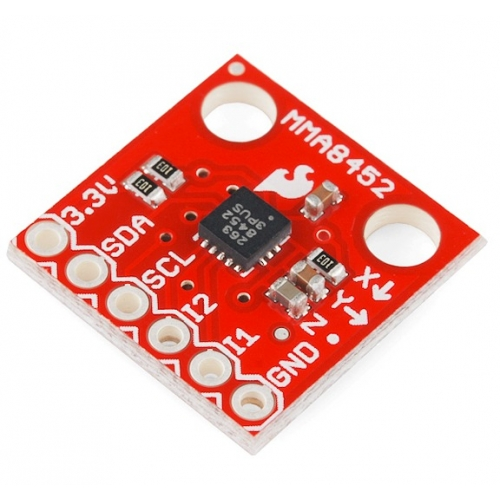
\includegraphics[width=0.3\textwidth]{Figures/accelerometer.jpg}
  \caption{Circuito MMA8452Q alambrado en un PCB.}
  \label{fig:accel}
\end{figure}

Asegúrese de \textbf{alimentar correctamente el circuito}, de lo contrario, el circuito podría dañarse permanentemente. Es muy recomendable que el sensor se coloque \textbf{horizontalmente y con el eje X alineado con el eje sagital del robot}. 

\subsection{Biblioteca para el sensor MMA8452Q}

El circuito MMA8452Q utiliza comunicación I2C para enviar las lecturas, por lo que tendría que programarse este protocolo en el nodo del Arduino, sin embargo, el fabricante proporciona una biblioteca para facilitar dicha comunicación. 

Descarge las bibliotecas para Arduino de la dirección \url{https://cdn.sparkfun.com/assets/learn_tutorials/2/4/9/SFE_MMA8452Q-library.zip}. Siga las instrucciones contenidas en la página \url{https://learn.sparkfun.com/tutorials/mma8452q-accelerometer-breakout-hookup-guide/example-code} para instalar y utilizar la biblioteca. 

\subsection{Nodo en el Arduino que publica los valores de aceleración}
Implemente un nodo en el Arduino que publique un tópico tipo \texttt{std\_msgs::Float32MultiArray} con el nombre \texttt{/minirobot/hardware/sensors} que contenga las lecturas del acelerómetro, además de todos los sensores construidos en las prácticas 4 y 5. El tamaño del arreglo de flotantes contenido en el mensaje \textbf{debe ser 15} y las lecturas de los sensores deben estar en el siguiente orden (ver prácticas 4 y 5 para los demás sensores): 

\begin{verbatim}
  {SD0 SD1 SD2 SD3 SD4 SD5 SD6 SD7   AccelX AccelY AccelZ   SLL  SLR  ST  SB}
\end{verbatim}

El acelerómetro puede reportar las lecturas de dos formas: \textit{raw data} y \textit{calculated data}. La primera reporta la aceleración como un entero de 12 bits y la segunda como un flotante en múltiplos de $g$. Los datos \textbf{deben reportarse como múltiplos de $g$}.

Por ejemplo, suponga que el acelerómetro está en reposo, en posición horizontal. Dado que siempre se tiene ruido en las mediciones, las lecturas de los tres ejes podrían ser $[0.0031,\;0.0041,\;0.99976]$. Si además los sensores SD0, SD2 y SD3 detectan objetos cercanos, los voltajes de los sensores de luz son 3.5V y 4.5V, la batería tiene un nivel de 8.0V y el sensor de temperatura entrega una salida de 0.8V, entonces, dado que el Arduino Uno tiene un ADC de 10 bits alimentado a 5V, el contenido del arreglo debería ser (recuerde que la batería pasa por un divisor de voltaje):
\begin{verbatim}
  {0  1  0  0  1  1  1  1  0.0031  0.0041  0.99976  717  922  164  819}
\end{verbatim}

con lo que la GUI desplegará algo como lo que se muestra en la figura \ref{fig:Example}. Para correr la GUI y visualizar los datos, en una nueva terminal, ejecute el comando

\begin{lstlisting}[language=bash]
$  rosrun mini_robot_gui mini_robot_gui_node
\end{lstlisting}

\begin{figure}
  \centering
  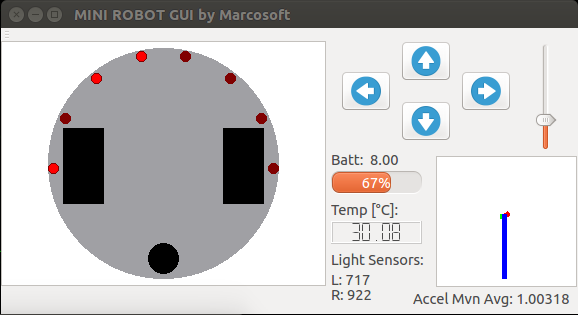
\includegraphics[width=0.7\textwidth]{Figures/SensorExample.png}
  \caption{Ejemplo de lectura de sensores.}
  \label{fig:Example}
\end{figure}

\subsection{Cambio de \textit{baudrate} en el Arduino}
Para el correcto funcionamiento del nodo del Arduino es necesario incrementar el \textit{baudrate} para asegurar que los datos se transmitan con suficiente rapidez y no haya pérdida de paquetes. 

Cambie el \textit{baudrate} del nodo del Arduino a 500000 bps agregando la línea 
\begin{lstlisting}
nh.getHardware()->setBaud(500000);
\end{lstlisting}
dentro de la función \texttt{setup()}, antes de llamar a la función \texttt{nh.initNode()}. Se asume que \texttt{nh} es el nombre de la variable de tipo \texttt{ros::NodeHandle}.

El nodo \texttt{serial\_node.py} debe ejecutarse con el comando
\begin{lstlisting}
$  rosrun rosserial_python serial_node.py _port:=/dev/ttyACM0 _baud:=500000
\end{lstlisting}
Asegúrese de seleccionar el puerto \texttt{tty} correcto. 

\subsection{Nodo para filtrado y cálculo de velocidad}

Programe un nodo, para ejecutarse en la computadora de escritorio o laptop, que se suscriba al tópico \texttt{/minirobot/hardware/sensors}. 

En este nodo, implemente un filtro pasa-banda de cuarto orden o superior, con frecuencias de corte de 0.5Hz y 5Hz, para filtrar la señal de aceleración en el eje $X$ únicamente. Puede utilizarse el comando \texttt{butter} incluido en el \textit{Signal Processing Toolbox} de MATLAB. Este comando devuelve dos arreglos de valores $[B,A]$ que corresponden a los coeficientes $b_k$ y $a_k$ de los polinomios en el numerador y denominador, respectivamente, de la ecuación (\ref{eq:Transfer}). 

El comando \texttt{butter} diseña un filtro digital empleando frecuencias de corte normalizadas, es decir, valores en [0,1], donde 1.0 corresponde a la mitad de la frecuencia de muestreo. Por lo tanto, para obtener la banda de 0.5-5.0Hz, las frecuencias de corte deben seleccionarse considerando la frecuencia de muestreo del nodo que se está implementando. Recuerde que esta frecuencia se fija con la clase \texttt{ros::Rate}.

En las ecuaciones (\ref{eq:Transfer}) y (\ref{eq:DiffEq}), la señal $x[n]$ corresponde a la aceleración (en el eje $X$) sin filtrar, y la señal $y[n]$ es la aceleración ya filtrada. Para obtener dicha señal filtrada, basta con despejar $y[n]$ de la ecuación (\ref{eq:DiffEq}), con lo que se obtiene la señal de salida en el tiempo actual, en términos de la entrada actual y salidas y entradas anteriores. 

En este mismo nodo, estime la velocidad en el eje $X$ mediante la integración numérica de la aceleración por el método del trapecio. Recuerde que en la ecuación (\ref{eq:Integral}), $\Delta t$ es el periodo de muestreo, que se fija con la clase \texttt{ros::Rate}. Nótese que para el diseño del filtro se requiere la \textbf{frecuencia} de muestreo, mientras que para la integración se utiliza el \textbf{periodo} de muestreo. 

Publique la señal de aceleración filtrada en el tópico \texttt{/minirobot/filtered\_accel}, de tipo \texttt{std\_msgs::Float32}. También publique la velocidad estimada en un tópico del mismo tipo con nombre \texttt{/minirobot/estimated\_speed}.

\subsection{Visualización de la velocidad y aceleración}
Para graficar la velocidad y aceleración en función del tiempo se utilizará el paquete \texttt{rqt\_plot}.

Para instalar el paquete, en una terminal teclee los siguientes comandos
\begin{lstlisting}{language=bash}
$  sudo apt-get install ros-indigo-rqt
$  sudo apt-get install ros-indigo-rqt-common-plugins
\end{lstlisting}

Ejecute el nodo del Arduino y el nodo de la subsección anterior. En otra terminal, teclee el siguiente comando
\begin{lstlisting}{language=bash}
$  rqt_plot /minirobot/filtered_accel /minirobot/estimated_speed
\end{lstlisting}
Aparecerá una gráfica con los valores de ambas señales.

\section{Evaluación}
\begin{itemize}
\item Los valores de aceleración deben mostrarse correctamente en la GUI. Al rotar al robot debe notarse claramente un cambio en la GUI por la componente de gravedad.
\item Todos los sensores, tanto el acelerómetro, como los de las prácticas anteriores, deben estar montados en el robot y funcionando correctamente. 
\item El correcto funcionamiento del filtro y el integrador se verificará mediante las gráficas desplegadas en el \texttt{rqt\_plot}.
\item Se girará al robot de modo que la componente de gravedad coincida con el eje $X$ para verificar el funcionamiento del filtro pasa-banda. 
\end{itemize}

\end{document}

%%% Local Variables:
%%% mode: latex
%%% TeX-master: t
%%% End:
